\documentclass{beamer}
\usepackage[utf8]{inputenc}
\usepackage{listings}
\usepackage{listingsutf8}
\usepackage{hyperref}
\usepackage{wrapfig}
\usepackage[absolute,overlay]{textpos}

\usetheme{Berkeley}

\title{NodeMCU}
\author{Fabiano Sardenberg Kuss}
\date{\today}


\lstset{
    language=c++,
    extendedchars=false,
    backgroundcolor=\color{gray!30},
    framextopmargin=2pt,
    framexbottommargin=2pt,
    rulecolor=\color{black!30},
    inputencoding=utf8
}


\begin{document}

\section{Introdução}

\begin{frame}[fragile, t]
\frametitle{Introdução}

A plataforma NodeMCU é uma placa open source baseada nas funcionalidade providas pelo chip de 
baixo custo com suporte a redes sem fio 802.11 ESP8266 que utiliza o microprocessador Xtensa.

Esta plataforma oferece um ambiente adequado para o desenvolvimento de dispositivos que 
implementam funcionalidades para atuarem em um conceito de IoT de forma simples. Pode
ser visto como uma evolução da estratégia de desenvolvimento utilizando Arduino

\begin{picture}(0,0)
    \put(20, -75){
    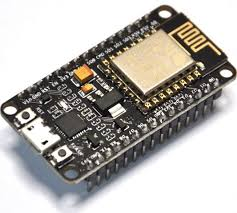
\includegraphics[scale=0.4]{imgs/nodeMCU.png}
    }
    \put(150, -60){
    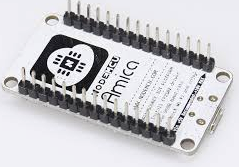
\includegraphics[scale=0.4]{imgs/back_node_mcu.png}
    }
\end{picture}

\end{frame}

\begin{frame}[fragile, t]
\frametitle{Apresentando a Placa}


\begin{picture}(0,225)
    \put(20, 15){
    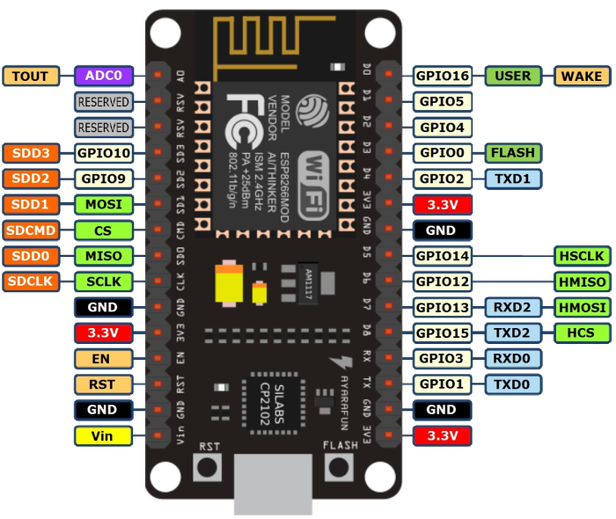
\includegraphics[scale=0.4]{imgs/pinout.png}
    }
\end{picture}

\end{frame}

\begin{frame}[fragile, t]
\frametitle{ESP8266}

\begin{picture}(0,0)
    \put(120, -200){
    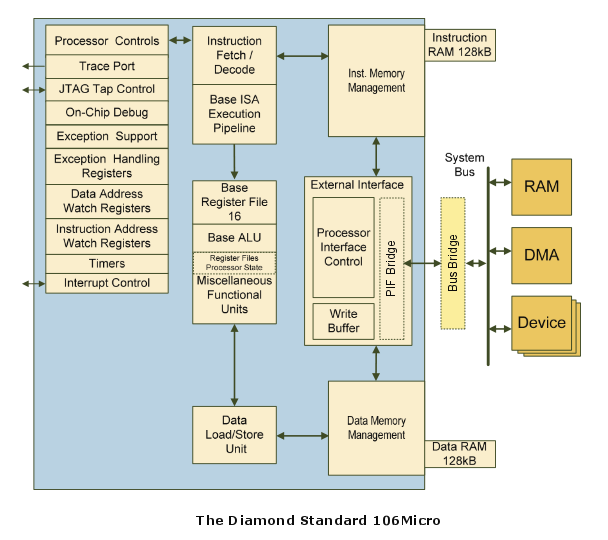
\includegraphics[scale=0.3]{imgs/xtensa-l106.png}
    }
\end{picture}


\begin{itemize}
\item Microcontrolador: Xtensa L106 (32-bit) 80Mhz
\item Memória Interna: 128K para instruções; 128K para dados
\item Memória Flash: 4Mb.
\item I/O: 16 Pinos GPIO
\item Tensão: 3.3 VDC
\item WI-FI: 802.11 b/g/n
\end{itemize}

\end{frame}


\begin{frame}[fragile]
\frametitle{Sintaxe básica}

Referência da linguagem:
https://www.lua.org/manual/5.2/pt/manual.htm

Algumas características:

\begin{itemize}
\item Dinâmicamente tipada
\item Variáveis sempre globais
\item Tipo table para qualquer tipo de array
\end{itemize}


\end{frame}


\begin{frame}[fragile]
\frametitle{Sintaxe básica}

Operadores:

\begin{itemize}
\item + adição  
\item - subtração
\item * multiplicação
\item / divisão
\item \% módulo
%\item ^ exponenciação
\end{itemize}


Operadores Lógicos:
\begin{itemize}
\item == comparador igualdade  
\item ~= comparador desigualdade
\item or 
\item and 
\item false 
\item true
\item nil Valor nulo
\end{itemize}

\end{frame}

\begin{frame}[fragile]
\frametitle{Sintaxe básica}
Algumas funções relevantes:

\begin{itemize}
\item tonumber(var) 
\item strlen(str)
\item type(var) --Retorna o tipo da variável
\item return 
\end{itemize}

Criando uma função:

f = function () corpo end

\end{frame}



\begin{frame}[fragile]
\frametitle{I/O}
Utiliza o operador : para manter o controle da operação utilizando uma sintaxe
mais simples.

\begin{lstlisting}
-- Sem arquivo fecha saída padrão
o.close ([file])
file:close([file])

--Intera sobre as linhas
io.input():lines()
\end{lstlisting}

Pode ser utilizado para socket como por exemplo 

\begin{lstlisting}
srv=net.createServer(net.TCP)
srv:listen()
\end{lstlisting}

\end{frame}

\begin{frame}[fragile]
\frametitle{Programando em Lua}

Download da ferramenta que permite comunicação serial usando Python
\tiny
\begin{lstlisting}
git clone https://github.com/pyserial/pyserial.git
\end{lstlisting}
\normalsize
Download da ferramenta de flash esptool.py em
\tiny
\begin{lstlisting}
git clone https://github.com/espressif/esptool
\end{lstlisting}

\normalsize
Copiar a pasta serial de pyserial-2.7

\tiny
\begin{lstlisting}
cp -r pyserial/pyserial-2.7/serial para a pasta esptool/
\end{lstlisting}

\normalsize
Compilar o próprio módulo ou fazer download de um módulo pronto de https://github.com/nodemcu/nodemcu-firmware/releases
Para a compilação será necessário 

Copiar o firmware para o dispositivo
\tiny
\begin{lstlisting}
./esptool.py -p /dev/ttyUSB0 write_flash 0x00000 \
~/Downloads/nodemcu_float_0.9.6-dev_20150704.bin
\end{lstlisting}
\end{frame}

\begin{frame}[fragile]
\frametitle{Oi mundo}
Escrever um oi mundo em lua
\tiny
\begin{lstlisting}

while true do
   print("Oi Mundo")
   tmr.delay(1000 * 1000)
end
\end{lstlisting}

\normalsize
Copiar o programa para o dispositivo

\tiny
\begin{lstlisting}
./luatool.py --port /dev/ttyUSB0  --src /tmp/script.lua --dofile
\end{lstlisting}
\end{frame}

\begin{frame}[fragile]
\frametitle{Comunicando com a serial}


Para comunicar com a porta serial para visualizar o resultado é possível utilizar um script python
lembrando que a pasta serial tem que estar no mesmo diretório que o script

\tiny
\begin{lstlisting}
import serial
ser = serial.Serial('/dev/ttyUSB0', 9600, timeout=1)
for i in range(0,10):
    print ser.readline()
\end{lstlisting}
\end{frame}

\begin{frame}[fragile]
\frametitle{Conectar em um AP}

Criando uma aplicação conectada ao Access Point

\tiny
\begin{lstlisting}
wifi.setmode(wifi.STATION)
wifi.sta.config("SSID","senha")

ip, nm, gw=wifi.sta.getip()

while true do
   print("\nIP Info:\nIP Address: "..ip.." \nNetmask: "..nm.." 
\nGateway Addr: "..gw.."\n")
   tmr.delay(2000*1000)
end
\end{lstlisting}
\end{frame}

\begin{frame}[fragile]
\frametitle{Requisições HTTP}

Atendendo requisições HTTP

\tiny
\begin{lstlisting}
srv=net.createServer(net.TCP)
srv:listen(80,function(conn)
  conn:on("receive",function(conn,payload)
    print(payload)
    conn:send("<h1>OLA ALUNO DO MINICURSO</h1>")
  end)
  conn:on("sent",function(conn) conn:close() end)
end)

\end{lstlisting}
\end{frame}


\begin{frame}[fragile]
\frametitle{Aplicação completa}

WEB e LED
\tiny
\begin{lstlisting}
LED_PIN = 1

gpio.mode(LED_PIN, gpio.OUTPUT)

wifi.setmode(wifi.STATION)
wifi.sta.config("pereskuss","meloquita")

ip, nm, gw=wifi.sta.getip()

print("\nIP Info:\nIP Address: "..ip.." \nNetmask: "..nm.." 
\nGateway Addr: "..gw.."\n")
tmr.delay(2000*1000)

srv=net.createServer(net.TCP)
srv:listen(80,function(conn)
  conn:on("receive",function(conn,payload)
    print(payload)
    conn:send("<h1>OLA ALUNO DO MINICURSO</h1>")
    gpio.write(LED_PIN, gpio.HIGH)
    tmr.delay(2000*1000)
    gpio.write(LED_PIN, gpio.LOW)
  end)
  conn:on("sent",function(conn) conn:close() end)
end)
\end{lstlisting}

\end{frame}

\begin{frame}[fragile]
\frametitle{Aplicação completa (Continuação)}

\tiny
\begin{lstlisting}
get={}

if string.find(valor, "GET") == 1 then
print("OK")
end

for w in string.gfind (valor, "%S+") do
    table.insert(get, w)
end

qstring = get[2]

init=string.find(qstring, "?")

substr = string.sub(qstring, init+1, string.len(qstring))


for w, k in string.gfind(qstring, '([^&=?]-)=([^&=?]+)' ) do
print(w, k)
end

\end{lstlisting}
\end{frame}

\begin{frame}[fragile]
\frametitle{Software Livre}
\tiny
\begin{lstlisting}
LED_PIN = 1

gpio.mode(LED_PIN, gpio.OUTPUT)

wifi.setmode(wifi.STATION)
wifi.sta.config("pereskuss","meloquita")

ip, nm, gw=wifi.sta.getip()

print("\nIP Info:\nIP Address: "..ip.." \nNetmask: "..nm.." 
\nGateway Addr: "..gw.."\n")
tmr.delay(2000*1000)

srv=net.createServer(net.TCP)
srv:listen(80,function(conn)
  conn:on("receive",function(conn,payload)
    print("PROCESS QS")
    for w, k in string.gfind(payload, '([^&=?]-)=([^&=?]+)' ) do print(w, k) end
    conn:send("<h1>OLA ALUNO DO MINICURSO</h1>")
    
    gpio.write(LED_PIN, gpio.HIGH)
    tmr.delay(2000*1000)
    gpio.write(LED_PIN, gpio.LOW)
  end)
  conn:on("sent",function(conn) conn:close() end)
end)
\end{lstlisting}
\end{frame}
\end{document}
